\section{Network Analysis}\label{sec:network_analysis}
\subsection{Building the protein-to-protein graph}\label{subsec:protein_to_protein_graph}
Starting from the interaction dataset built after the geneset expansion (as we have seen in \autoref{sec:geneset_expansion}) we developed our protein-to-protein network thanks to the networkx\footnote{https://github.com/networkx/networkx} python package. First we inserted the nodes into the graph and named them with the protein they represent, and, at the same time we "colored" them with the disease pathways they belong to. Then, we created the edges from the interaction dataset and we weighted them based on the number of shared diseases (the ones retrieved during the pathway enrichment explained in \autoref{sec:pathway_enrichment}) between couple of nodes.
\vspace{3mm}

We noticed that a relevant number of nodes/proteins does not belong to any disease, more precisely $5101$ of the $13010$ proteins. Since we did not want to end with possibly a non-connected graph, we decided to keep them. The same can also be seen for the edges, since we have observed that $45000$ of them had no shared diseases between the couple of nodes they connect, but the same reasoning we did for the nodes stands for them, so we kept them too. \autoref{fig:nodes_edges_no_disease} shows the how we computed such nodes and edges after building our protein-to-protein graph.
\begin{figure}[H]
    \centering
    \subfloat[Nodes with no color/disease]{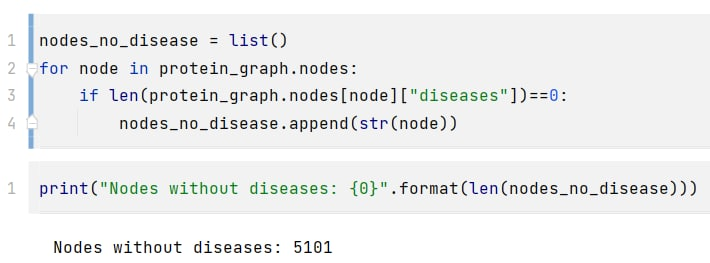
\includegraphics[width=0.5\linewidth]{images/nodes_no_diseases.jpg}}
    \subfloat[Edges with no weight/disease]{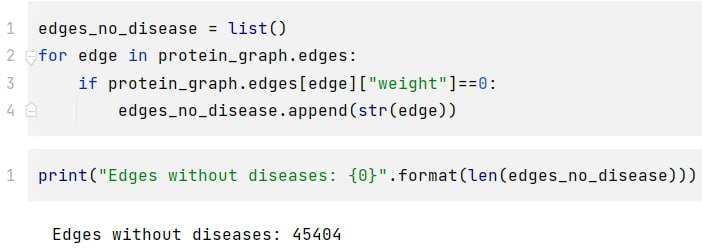
\includegraphics[width=0.5\linewidth]{images/edges_no_diseases.jpg}}
    \caption{Jupyter cells that compute the number of nodes and edges that do not belong to any disease pathway.}
    \label{fig:nodes_edges_no_disease}
\end{figure}

\subsection{Disease network metrics}\label{subsec:disease_metrics}
Once we built the protein-to-protein graph (we talked about it in \autoref{subsec:protein_to_protein_graph}) we computed some of the metrics proposed by Agrawal et al. \cite{agrawal2018} to have a better overview on the effect of each disease pathway on our newly built graph.
\paragraph{Size of largest pathway component} \textit{Fraction of disease proteins that lie in the disease's largest pathway component (i.e., the relative size of the largest connected component (LCC) of the disease)} \cite{agrawal2018}. It indicates how prevalent is the biggest component of genes inside a disease pathway and, therefore, how its genes are connected between them.
\paragraph{Distance of pathway components} \textit{For each pair of pathway components, we calculate the average shortest path length between each set of proteins, and then, the average of this is taken over all pairs of the components} \cite{agrawal2018}. Even though this metric tells us how distant are a disease's genes and, therefore, how long is the path between them, it is not valuable in our case since, as we explained at the end of \autoref{sec:geneset_expansion}, our graph is centered around the SON gene and, for that reason, the maximum distance of each node from one another is $4$.

\subsection{Biomarkers identification}\label{subsec:biomarkers}
A main issue, not the hardest but for sure the most annoying and tedious one, was related to plotting the graph, which had too many nodes and interactions to be properly drawn. Moreover, we were interested in knowing which were the biomarkers, the "central" nodes of our graph, the ones that have more "impact" on its connectivity. Solving the latter would have also made the plotting far easier, so we it was a logical step at the end of our network analysis.
\vspace{3mm}

By using the centrality algorithm based on the nodes' degree from the networkx package, we made a method that retrieves a user-specified number of biomarkers plus one protein of their choice (in our case the SON gene). \autoref{fig:biomarkers} shows the $30$ biomarkers identified whose centrality is the ratio between the node degree over the entire number of nodes that compose the protein-to-protein graph.
\begin{figure}[H]
    \centering
    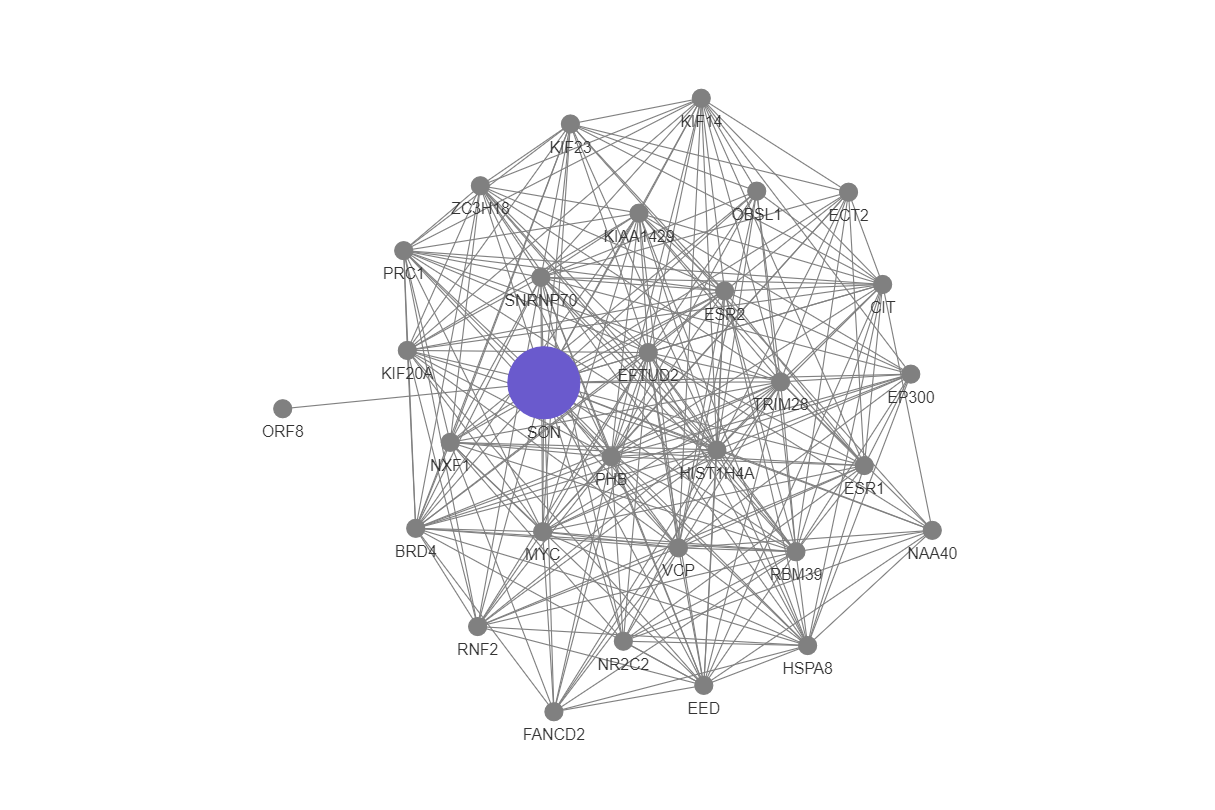
\includegraphics[width=1\linewidth]{images/plots/plot_biomarkers.png}
    \caption{Biomarkers with the SON gene highlighted.}
    \label{fig:biomarkers}
\end{figure}